\chapter{Active learning \label{ch:al}}

Active learning is a subset of machine learning wherein an algorithm is 
``trained'' on labeled data instances in order to learn from and make 
predictions on the data.  Consider a large set of unlabeled data $X$ with a 
hidden label from a finite set $Y$ that can be queried from some human 
``oracle''; we would like to learn a good classifier of the data, some mapping 
$h: X \rightarrow Y$ from the set $\mathcal{H}$ without making too many 
queries~\cite{dasgupta2011}. Active learning is the process of intelligently 
selecting the queries (a constrained resource) to learn as much as possible. 
When a learning algorithm is allowed to choose its next query, it performs 
better with less training~\cite{settles2010}. To put it more concretely, the 
error (a measurement of the difference between the predicted labels and the 
``true'' labels) converges to zero faster. This property is especially 
desirable when labeled data are difficult, time-consuming, or computationally 
expensive to obtain. Stage one of the VS (Section~\ref{sec:visualizer:al}) is 
one such classification task where $Y\in\{$interesting, non-interesting$\}$. 
Classification and filtering tasks are both tedious and redundant, which 
necessitates intelligent selection of queries~\cite{settles2010}. What follows 
is an active learning literature review in Section~\ref{sec:al:litreview}, an 
overview of active learning methods and their algorithms in 
Section~\ref{sec:al:methods}, and a simulation study in 
Section~\ref{sec:al:simulations} to determine the method that is best-suited 
for usage with the VS in Chapter~\ref{ch:usage}'s equity application.

\section{Literature review}
\label{sec:al:litreview}

It is important to consider the main framework in which the learning algorithm 
selects a query from unlabeled data. There are three different 
scenarios in which the learner may request queries as described by 
Settles~\cite{settles2010}:
 
\tablespacing
\begin{enumerate}
	\item \textbf{Membership query synthesis}: The learner may select a query 
	from any unlabeled samples in $X$.
	\item \textbf{Stream-based selective sampling}: An unlabeled sample is 
	randomly selected from $X$, and the learner decides whether to query or not.
	\item \textbf{Pool-based sampling}: $k$ unlabeled samples are randomly 
	selected from $X$, and the learner picks one to query.
\end{enumerate}
\bodyspacing

\noindent While the methods above may apply to many different active learning 
environments, the specific situation for the VS is \textit{pool-based selective 
sampling}. Because it is computationally expensive to extract features from 
every single $n\choose2$ plot (see 
Section~\ref{sec:visualizer:scatterplot:features}), membership query synthesis 
is not an option. While stream-based selective sampling may work, it has a 
similar problem because there are no constraints
on the number of samples that the algorithm may choose to discard. 

The next problem, then, is to determine the informativeness of unlabeled 
instances that are presented by the situations above. This is the crux of 
active learning as it allows for intelligent selection of queries.
Dasgupta identifies two different approaches to active learning that are 
fundamental to the process of query selection~\cite{dasgupta2011}: 

\tablespacing
\begin{enumerate}
	\item \textbf{Efficient search through hypothesis space $\mathcal{H}$}: 
	The idea is to select a query that shrinks $\mathcal{H}_t$, the set of all 
	possible classifiers at time $t$ that explain the labeled data, as much as 
	possible. 
	\item \textbf{Exploiting cluster structure in data}: 
	The idea is to cluster the data and select queries based on cluster 
	structure (i.e. query from each cluster). While clusters may be split over 
	time if they are discovered to be non-homogenous, a learner may leverage 
	situations where clusters are fairly homogeneous in order to classify 
	points by propagating a node's label to its neighbors. 
\end{enumerate}
\bodyspacing

\noindent Uncertainty sampling, query by committee, and query by bagging are 
active learning algorithms that are a form of the aforementioned efficient 
search through the hypothesis space. These algorithms may be found in 
Sections~\ref{sec:al:methods:uncertainty} to~\ref{sec:al:methods:bagging} 
respectively. We also present a clustering partitioning algorithm in 
Section~\ref{sec:al:methods:clustering} that seeks to exploit the clustering  
structure in the data.

\section{Overview of active learning methods}
\label{sec:al:methods}

In this section, we present algorithms for specific active learning methods and 
a reference to its implementation in the appendix. The 
\texttt{activelearning} package by \texttt{ramhiser}~\cite{ramhiser2015} has 
adapted much of the methods reviewed in Settles' paper~\cite{settles2010}. As 
such, most of the implementation code has been adapted and reworked (with 
substantial components written from scratch) from the 
\texttt{activelearning} package, which is too general for our purposes.

\subsection{Uncertainty sampling}
\label{sec:al:methods:uncertainty} 

In uncertainty sampling, the active learner selects the query $q$ that it is 
most uncertain on how to label; in other words, the algorithm queries the label 
that has the highest posterior probability~\cite{lewis1994}. With binary 
classification as is the case with the VS (either ``visually correlated'' or 
``not visually correlated''), this reduces to the case of querying the instance 
whose posterior probability of being ``visually correlated'' is closest to 
0.5~\cite{lewis1994}. While the uncertainty sampling algorithm presented in 
Algorithm~\ref{alg:al:methods:uncertainty} follows this 
methodology and may subsequently only be used with classification models that 
are able to encompass posterior probability computations, there has been much 
work done to expand uncertainty sampling to non-probabilistic classifiers such 
as decision trees and nearest-neighbor~\cite{settles2010}.

Uncertainty sampling is simple but not without problem. Given a multi-label 
classification problem (labels $k > 2$), uncertainty sampling only 
considers the information about the most probable label $i$ and ignores the 
other possible labels $j \in \{1,...,k\}\backslash i$. ``Margin sampling'' and 
``entropy'' are variants that try to solve for these problems, but 
both reduce to the scheme of querying from the sample with a posterior 
probability closest to 0.5 when $k=2$ (binary 
classification)~\cite{settles2010}.

We have developed an algorithm for uncertainty sampling based on the literature 
review (see Appendix~\ref{sec:appendicies:al:uncertainty} for code):

\tablespacing
\begin{algorithm}[H]
	\caption{Uncertainty sampling (as described by 
	Settles~\cite{settles2010})}\label{alg:al:methods:uncertainty}
	\begin{algorithmic}[1]
		\Procedure{}{$X$ is a $n\times d$ matrix of $d$ observations of all $n$ 
		variables, $y$ is an $n$-length vector of labels for each variable in 
		$X$ ($y_i$=N/A when $X_{i,}$ has no label)}
		\State $\textit{tout} \gets 
		\text{train}(X^{\text{labeled}},y^{\text{labeled}},\text{classification 
		model})$
		\State $p \gets 
		\text{predict}(\textit{tout},X^{\text{unlabeled}},
		\text{posterior prob. = TRUE})$
		\State \textbf{loop from} $i=1$ \textbf{to} len($p$):
		\State \indent $p_i \gets |p_i-0.5|$
%		\If {$\textit{string}(i) = \textit{path}(j)$}
%		\State $j \gets j-1$.
%		\State $i \gets i-1$.
%		\State \textbf{goto} \emph{loop}.
%		\State \textbf{close};
%		\EndIf
		\State \textbf{return} where($p==\min{(p)}$)
		\EndProcedure
	\end{algorithmic}
\end{algorithm}
\bodyspacing

\noindent By searching for the most ``uncertain'' point, uncertainty sampling 
is able to further refine the classifier as the oracle must label the point 
either ``visually correlated'' or ``not visually correlated''. This can be 
viewed as a search within the hypothesis space $\mathcal{H}$ that contains 
multiple classifiers, instances of a single classification model.








\subsection{Query by committee}
\label{sec:al:methods:qbc}

Query by committee is another case of efficient search through the hypothesis 
space. In query by committee, a ``committee'' of classification models are 
trained on the  current labeled instances.  Each model represents a competing 
hypothesis, and its prediction for an unlabeled query candidate $q$ is a 
``vote'' of weight one on $q$; the most disagreeable candidate is then 
queried~\cite{settles2010}. Settles reviews various methods for initial 
committee selection by the active learner (for both probabilistic and 
non-probabilistic models), though our implementation of QBC 
(Appendix~\ref{sec:appendicies:al:qbc}) allows the user to specify the 
committee members~\cite{settles2010}. 

The basic algorithm is as follows:

\tablespacing
\begin{algorithm}[H]
	\caption{Query by committee (as described by 
	Settles~\cite{settles2010})}\label{alg:al:methods:qbc1}
	\begin{algorithmic}[1]
		\Procedure{}{$X$ is a $n\times d$ matrix of $d$ observations 
		of all $n$ variables, $y$ is an $n$-length vector of labels for each 
		variable in $X$ ($y_i$=N/A when $X_{i,}$ has no label). Let $C$ be the 
		vector of all committee members i.e. classification models}
		\State \textbf{loop from} $i=1$ \textbf{to} len($C$):
		\State \indent $\textit{tout}_{i} \gets 
		\text{train}(X^{\text{labeled}},y^{\text{labeled}},C_i)$
		\State \indent $p_{i,} \gets 
		\text{predict}(\textit{tout}_i,X^{\text{unlabeled}})$
		\State $d \gets \text{disagreement}(p)$
		\State \textbf{return} where($d==\max{(d)}$)
		\EndProcedure
	\end{algorithmic}
\end{algorithm}
\bodyspacing

\noindent While it is simpler to maintain the same committee 
throughout, it would be more informative to prune the committee as the 
algorithm proceeds; it may simply be the case that a model is ill-suited for 
the problem at hand and consistently returns predictions that skew the voting 
procedure. Subsequently, a model is removed from the committee if its 
predictions are consistently out-of-line with whatever the ``true'' label of 
$q_t$ (the next query point decided and then queried at time $t$) turns out to 
be. It is important to note that the ``true'' label is not known until 
\textit{after} the algorithm has returned the index of $q_t$. In the VS, this 
index corresponds to the next pairwise scatter plot to show the 
user and query. Subsequently, the committee from $t$ 
is pruned at time $t+1$ at the start of the algorithm using the label retrieved 
from time $t$. The pruning function should only 
be run after a good number of iterations (where each iteration results in a 
query) have passed to allow the error ratios to converge (Otherwise, there is 
no room for learning). In our implementation, we begin using the pruning 
algorithm after $iter/2$ queries where $iter$ is the query budget (the maximum 
number of queries allowed).
Furthermore, the query by committee methodology described by Settles only uses 
the committee to select $q$; thus, the committee is independent of the final 
classification model (in the VS, this is a random forest) once the budget has 
been used up~\cite{settles2010}. However, there may be merit in maintaining the 
final pruned committee as its own classification model after the budget has 
been used up. As a classification model, the pruned committee may label 
unlabeled instances via majority vote. Further details on implementation and a 
performance comparison may be found in the simulation study 
(Section~\ref{sec:al:simulations}). The revised algorithm is as follows (see 
Appendix~\ref{sec:appendicies:al:qbc} for code):

\tablespacing
\begin{algorithm}[H]
	\caption{Query by committee (revised framework)}\label{alg:al:methods:qbc2}
	\begin{algorithmic}[1]
		\Procedure{}{$X$ is a $n\times d$ matrix of $d$ observations of all $n$ 
		variables, $y$ is an $n$-length vector of labels for each variable in 
		$X$ ($y_i$=N/A when $X_{i,}$ has no label). Let $C$ be the vector of 
		all committee members i.e. classification models, $E$ be the average 
		error ratio of the respective 
		committee members (initialized to 0), $0<\epsilon<1$ be some threshold 
		for the error ratio, \textit{iter} be the total active learning 
		budget, and $t$ be the current iteration of QBC starting 
		at $t=1$}
		
		\Function{QBC}{}
		\State \textbf{loop from} $i=1$ \textbf{to} len($C$):
		\State \indent $\textit{tout}_i \gets 
		\text{train}(X^{\text{labeled}},y^{\text{labeled}},C_i)$
		\State \indent $p_{i,} \gets 
		\text{predict}(\textit{tout}_i,X^{\text{unlabeled}})$
		\State $d \gets \text{disagreement}(p)$
		\State \textbf{return} $j =$ where($d==\max{(d)}$)
		\EndFunction
		
		\Function{Oracle}{}
		\State \textbf{return} $l$, the label of $X_{j,}$
		\EndFunction
		
		\State $y_j \gets l$
		
		\Function{Prune }{When iteration $i \in [1,iter] > iter/2$, run 
		\textsc{Prune}}	
		\State $prune = [\ ]$ (empty vector)	
		\State \textbf{loop from} $i=1$ \textbf{to} len($C$):
		\State \indent \textbf{If} ($p_{i,j}==y_j$) \textbf{then} $iv = 0$ 
		\textbf{Else} $iv = 1$
		\State \indent $E_i = E_i + \frac{iv - E_i}{t}$
		\State \indent \textbf{If} $E_i>\epsilon$ \textbf{then} 
		$prune.\text{append}(i)$
		\State $t++$
		\State \textbf{return} $prune$
		\EndFunction
		
		\State \textbf{loop from} $i=1$ \textbf{to} len($prune$):
		\State \indent Delete $E_{prune_i}$, $C_{prune_i}$, $p_{prune_i,}$, 
		and $\textit{tout}_{prune_i}$
		
		\EndProcedure
	\end{algorithmic}
\end{algorithm}
\bodyspacing

Note that both Algorithm~\ref{alg:al:methods:qbc1} 
and~\ref{alg:al:methods:qbc2} contain a generic disagreement function, which 
measures the disagreement among the committee members. Let $Y$ be the set of 
all possible labels. There are two main methods of measuring disagreement 
described by Settles~\cite{settles2010}:

\tablespacing
\begin{enumerate}
	\item \textbf{Vote entropy}: The disagreement for query candidate $q$ is 
	computed
	$$d_{\text{VE}}(q) =-\sum\limits_{y \in Y} 
	\frac{V(y|q)}{\text{len}(C)} \log \frac{V(y|q)}{\text{len}(C)}$$
	\noindent where $0 \leq V(y|q) \leq \text{len}(C)$ is the number of votes 
	that label $y$ received for query candidate $q$. 
	The interested reader may refer to Dagan and 
	Engelson~\cite{dagan1995} for further details.
	
	\item \textbf{Kullback-Leibler divergence}: The disagreement for query 
	candidate $q$ is computed
	$$d_{\text{KL}}(q) = \frac{1}{\text{len}(C)} \sum\limits_{i =
	1}^{\text{len}(C)} \sum\limits_{y \in Y} 
	\text{P}_{C_i}(y|q) \log \frac{\text{P}_{C_i}(y|q)}
	{\text{P}_{C}(y|q)}$$
	\noindent Recall that $C$ is the vector of committee members. We can 
	interpret $\text{P}_{C}(y|q) = \frac{1}{\text{len}(C)} 
	\sum\limits_{k=1}^{\text{len}(C)} \text{P}_{C_k}(y|q)$ as the probability 
	that label $y$ will have the most votes for $q$, and 
	$\text{P}_{C_k}(y|q)$ as the probability that committee member $k$ votes 
	$y$ for $q$. The interested reader may refer to McCallum and 
	Nigam~\cite{mccallum1998} for further details.
\end{enumerate}
\bodyspacing

\noindent An implementation of vote entropy disagreement can be found in 
Appendix~\ref{sec:appendicies:al:entropy}. This function was imported from the 
\texttt{activelearning} package developed by 
\texttt{ramhiser}~\cite{ramhiser2015} and simply calls the \texttt{entropy} 
package in \texttt{R}.









\subsection{Query by bagging}
\label{sec:al:methods:bagging}

Query by bagging and boosting was proposed
as a way to improve the performance of a single classifier by forming a 
committee of classifiers trained on random (weighted, in the case of Boosting) 
subsets of the labeled data~\cite{abe1998}. 
Bagging uniformly samples $k$ subsets from the labeled data to form a committee 
of $k$ different classifiers, which are trained with the same classification 
model (e.g. random forest)~\cite{abe1998}. The unlabeled data with the most 
disagreement among the committee members is then selected as the next oracle 
query (see Section~\ref{sec:al:methods:qbc} for details on disagreement 
measures). The algorithm is as follows (see 
Appendix~\ref{sec:appendicies:al:bagging} for code):

\tablespacing
\begin{algorithm}[H]
	\caption{Query by bagging (as described by Abe and 
	Mamitsuka~\cite{abe1998})}\label{alg:al:methods:bagging}
	\begin{algorithmic}[1]
		\Procedure{}{$X$ is a $n\times d$ matrix of $d$ observations 
			of all $n$ variables, $y$ is an $n$-length vector of labels for 
			each variable in $X$ ($y_i$=N/A when $X_{i,}$ has no label). 
			$num\_class$ is the desired number of committee members (subsets to 
			sample). Let $r \in (0,1)$ such that 
			$r*\text{len}(X^{\text{labeled}})$ is the number of points to 
			randomly sample for each subset of the labeled set.}
		\State \textbf{loop from} $i=1$ \textbf{to} $num\_class$:
		\State \indent $idx \gets \text{unif\_sample}(\text{labeled}, 
		r*\text{len}(X^{\text{labeled}}) )$
		\State \indent $\textit{tout}_{i} \gets 
		\text{train}(X_{idx, },y_{idx},\text{classification model})$
		\State \indent $p_{i,} \gets 
		\text{predict}(\textit{tout}_i,X^{\text{unlabeled}})$
		\State $d \gets \text{disagreement}(p)$
		\State \textbf{return} where($d==\max{(d)}$)
		\EndProcedure
	\end{algorithmic}
\end{algorithm}
\bodyspacing

\noindent Since each iteration of the query selection is a new process of 
random committee training, there is no starting committee. Instead, what the 
user specifies is the classification model that each subset will be trained on. 
Subsequently, there is no need to (1) maintain error ratios to prune a starting 
committee or to (2) use majority vote with a pruned committee for the final 
fitted model over a random forest, which is the classification model for stage 
2 (Section~\ref{sec:visualizer:plotgeneration}).










\subsection{Min-max clustering}
\label{sec:al:methods:clustering}

The goal of the Min-Max Approach is to query points that are far from each 
other~\cite{vu2010}. This can be done by selecting a query that maximizes the 
minimal distance of each unlabeled query from the labeled set~\cite{vu2010}. 
In other words, 
$$\max\limits_{q \in X^{\text{unlabeled}}} \bigg( \min\limits_{k \in 
X^{\text{labeled}}} \bigg( \text{distance}(q,k) \bigg) \bigg)$$

Given natural clustering in the data, the active learner would be able to 
sample from each cluster with this methodology. If each cluster is fairly 
homogeneous, the final fitted classifier will be a good representation of the 
data set's ``true'' labels (Section~\ref{sec:al:litreview}). As such, min-max 
clustering is able to exploit the clustering structure of data but 
may perform more poorly (converge more slowly i.e. require more queries to get 
to a reasonable error level) in data sets that do not naturally form clusters. 
Naturally, there are two important considerations:

\tablespacing
\begin{itemize}
	\item \textbf{Initialization:} How does the active learner find the 
	clusters in the first place? Selecting points near the centers of the 
	clusters, which are the densest regions, allows the algorithm 
	to converge faster~\cite{vu2010}.
	
	\item \textbf{Query selection:} How does the active learner quantify the 
	distance between data points? Euclidean distance is a common metric of the 
	straight-line distance between points in the Euclidean space.
\end{itemize}
\bodyspacing

Vu \textit{et al.} proposed the creation of a $k$-nearest neighbors graph 
to measure the local density of each data point; the most dense points may be 
selected to initialize the active learner~\cite{vu2010}. Since the VS will be 
initialized randomly for reasons described in 
Section~\ref{sec:visualizer:al:initialization}, we do not concern ourselves too 
much with min-max clustering initialization; 
the interested reader may refer to~\cite{vu2010} for 
more of the mathematical details and a demonstration of viability. 
Instead, we present the simple algorithm for the actual active learning 
(querying) process (see Appendix~\ref{sec:appendicies:al:clustering} for code):

\tablespacing
\begin{algorithm}[H]
	\caption{Min-max clustering (as described by 
		Vu \textit{et al.}~\cite{vu2010})}\label{alg:al:methods:clustering}
	\begin{algorithmic}[1]
		\Procedure{}{$X$ is a $n\times d$ matrix of $d$ observations of all $n$ 
			variables, $y$ is an $n$-length vector of labels for each variable 
			in $X$ ($y_i$=N/A when $X_{i,}$ has no label)}
		\State \textbf{loop from} $i=1$ \textbf{to} len($y^{\text{unlabeled}}$):
		\State \indent $\min \gets \infty$
		\State \indent \textbf{loop from} $j=1$ \textbf{to} 
		len($y^{\text{labeled}}$):
		\State \indent \indent  $d \gets 
		\text{distance}(X_{i,}^{\text{unlabeled}},X_{j,}^{\text{labeled}})$
		\State \indent \indent \textbf{If} $(\min >d): \min \gets d$
		\State \indent $q_i \gets \text{min}$
		\State \textbf{return} where($q==\max{(q)}$)
		\EndProcedure
	\end{algorithmic}
\end{algorithm}
\bodyspacing
\section{Simulations}
\label{sec:al:simulations}

We utilize a simulation study in order to determine the method that is 
best-suited for usage with the VS in Chapter~\ref{ch:usage}'s equity 
application. To recap, these are key features of the visualization system that 
should be (and are) captured in the simulations:

\tablespacing
\begin{itemize}
	\item \textbf{Initialization (Section 
	~\ref{sec:visualizer:al:initialization}):} 
	Initializing the active learner begins with a random selection of $k$ data 
	that is presented to the oracle for classification. Each simulation is 
	initialized with 10 randomly selected data points.
	\item \textbf{Pool-based sampling (Section ~\ref{sec:al:litreview}):} After 
	initialization, $k$ unlabeled samples are randomly selected from $X$, and 
	the active learner picks one to query. Each simulation iteration (of the AL 
	algorithm) is presented 15 unlabeled points to query from.
	\item \textbf{Random forest 
	(Section~\ref{sec:visualizer:plotgeneration:tree}):} The VS's overall 
	classification model (for use when initialization and querying are 
	complete) is a random forest. Each active learning method in the 
	simulations optimize for the 
	final random forest classification model by utilizing random forests in 
	their selection process (excluding QBC due to the nature of the 
	algorithm). Instead, the QBC simulations have been run with a committee of 
	classification models that includes random forest (See 
	Section~\ref{sec:al:simulation:methods} for the full list). Furthermore, 
	the QBC simulations have been run with both (1) majority vote and (2) 
	random forest as the overarching classification, as well as (1) with 
	pruning and (2) without pruning.
	\item \textbf{Bivariate classification:} The classification of user 
	interests have two possible labels/levels: ``interesting'' and ``not 
	interesting''. The simulations also use data with two levels of 
	classification (Section~\ref{sec:al:simulation:data}).
\end{itemize}
\bodyspacing

\noindent Finally, it should be noted that each active learning algorithm is 
given a budget of 50 queries (50 progressive iterations of a single trial).

\subsection{Data}
\label{sec:al:simulation:data}
The data is taken from the MNIST database of handwritten digits 
(\url{http://yann.lecun.com/exdb/mnist/}). The digits $(0,1,...,9)$ have 
already been classified and may be visualized in the form of a $28\times 28$ 
pixel array; the darkness of each pixel is represented by a value from 0 
(light) to around 300 (dark). Each image has been transformed into a single 
784-length vector by ``unfurling'' each row and adding it to the last column of 
the row above it. For ease of use and computation efficiency, the data has been 
further compressed to a 196-length vector ($14\times 14$ pixel image). In order 
to maintain the condition of bivariate classification, two out of ten digits 
were selected. The digits 7 and 9 were selected as they are rather similar, 
making it more difficult for an active learning algorithm to correctly parse 
the data with few queries (As opposed to 1 and 0, which are very different on 
the visual plane). The MNIST training set contains 60,000 total data points 
while the testing set contains 10,000 total data points. This was far too many, 
so the simulator selects 250 random samples (125 of each digit) from the 
training set to make up the final data. The final dataset may be visualized in 
Figure~\ref{fig:al:simulations:data}. The functions for working with the MNIST 
data were adapted from file \texttt{gist:39760}~\cite{oconnor2008} and may be 
found in Appendix~\ref{sec:appendicies:al:simulations:data}.

\begin{figure}[htb]
	\begin{center}
		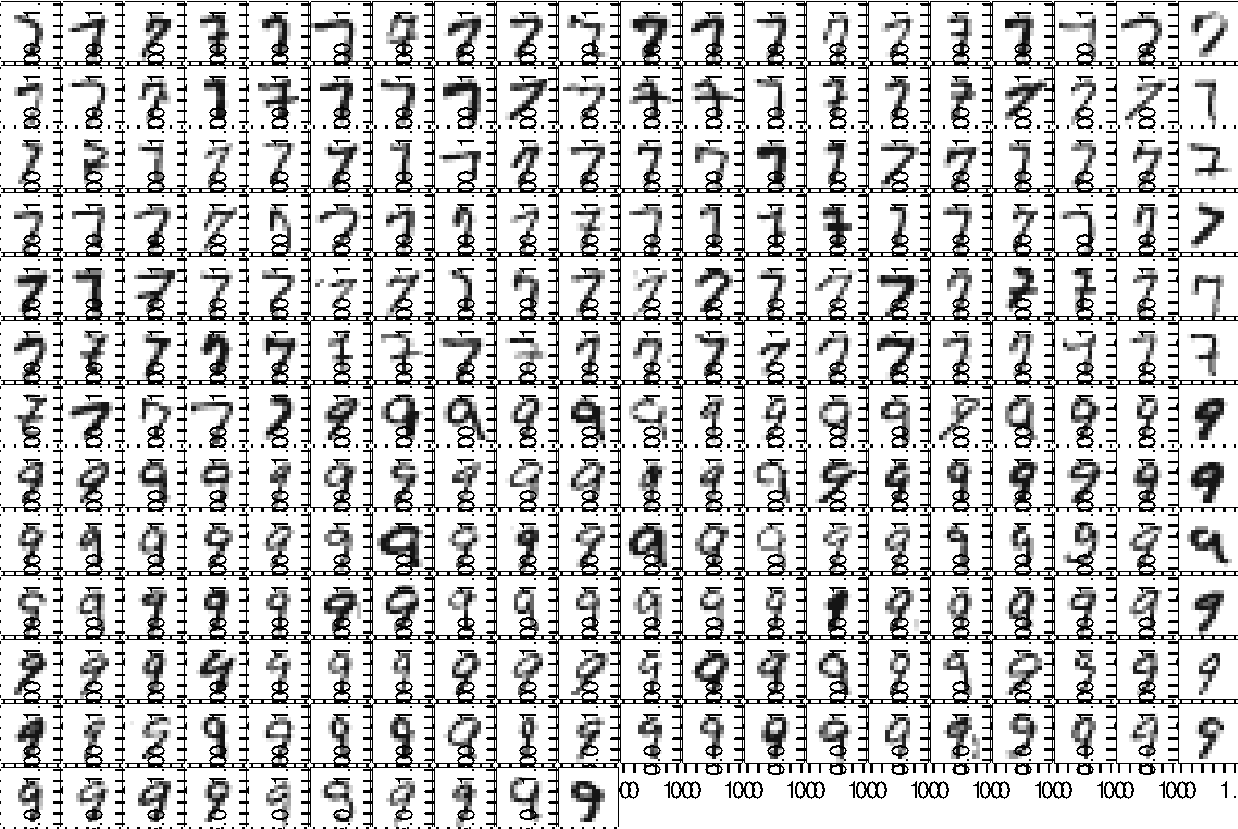
\includegraphics[width=1\linewidth]{ch-al/figures/data.pdf}
		\caption[MNIST data used in the simulations.]{MNIST data used in the 
		simulations. The digits 7 and 9 are relatively similar visually, making 
		the simulations more realistic as it is harder for the classificaiton 
		models to tell the difference.}
		\label{fig:al:simulations:data}
	\end{center}
\end{figure}

\subsection{Evaluation}
\label{sec:al:simulation:evaluation}
The performance of a learner at any given point in time (at any iteration 
\textit{i} of simulation number $k \in [1,25]$) is encapsulated in its error 
ratio $\epsilon$. That is, given the current labeled set, the \textbf{main 
classifier (Random Forest model)} is trained, and the entire dataset is 
predicted given the current classifier. The predictions are stored in an 
$n$-length vector $p$. 
We know the true labels ahead of time (thanks to the MNIST dataset), and they 
are stored in an $n$-length vector $y'$. The predictions are compared against 
the true labels and the error ratio of iteration $i$ is given by
$$\epsilon_i = \frac{1}{250} \bigg( \sum\limits_{z=1}^{250} 
\textbf{1}_{p_z \neq y'_z} \bigg)$$

\noindent where $\textbf{1}_{p_z \neq y'_z}$ is an indicator variable that is 1 
when $p_z \neq y'_z$ and 0 otherwise. These 50 error ratios then form one 
vector $\epsilon_s$, the result of trial 
$s$. To select the best active learning algorithm \textit{on average}, each 
algorithm's error ratios are averaged over 25 total trials. This helps offset 
the randomness of the initialization and pooling scheme. Then the final error 
ratio of an algorithm is given by
$$\epsilon = \frac{1}{25} \bigg( \sum\limits_{i=1}^{25} \epsilon_s \bigg)$$

The final framework for computing $\epsilon_s$, a single trial's vector of 
error ratios, is summarized as follows (This procedure is encapsulated by the 
simulation engine code in 
Appendix~\ref{sec:appendicies:al:simulations:simengine}):

\tablespacing
\begin{algorithm}[H]
	\caption{Computing $\epsilon_s$, a single trial's vector of error 
	ratios}\label{alg:al:simulation:evaluation}
	\begin{algorithmic}[1]
		\Procedure{}{$X$ is a $n\times d$ matrix of $d$ observations of all $n$ 
			variables, $y$ is an $n$-length vector of labels for each variable 
			in $X$ ($y_i$=N/A when $X_{i,}$ has no label). $y'$ is an 
			$n$-length vector of \textbf{true} labels for each variable in $X$. 
			$iter$ is the maximum number of queries allowed per trial}
		\State \textbf{loop from} $i=1$ \textbf{to} $iter$:
		\State \indent $idx \gets $ active\_learning\_method$(X,y,...)$
		\State \indent \textsc{Query} $X_{idx,}$
		\State \indent $tout \gets 
		\text{train}(X^{labeled},y^{labeled},\text{randomforest})$
		\State \indent $p \gets \text{predict}(tout,X)$
		\State \indent $res_i\gets \frac{\text{length}(\text{which}(p \neq y'))}
		{\text{length}(y')}$
		\State \textbf{return} $res$
		\EndProcedure
	\end{algorithmic}
\end{algorithm}
\bodyspacing

\subsection{Summary of methods}
\label{sec:al:simulation:methods}

What follows is a summary of the active learning methods used in the simulation 
with details such tuning parameter values.

\tablespacing
\begin{longtable}{p{0.15\linewidth} p{0.21\linewidth} p{0.18\linewidth} 
p{0.4\linewidth}}
	
	% First page heading
	\caption[Summary of simulation active learning methods.]{A summary of the  
	active learning methods tested in the simulation. *\textit{Note:} The 
	classification model is the main classification model that is used to fit 
	the error, not the classification model(s) used in the active learning 
	methods (those are parameters). 
	The classification model in the simulator is akin to the main 
	classification model in the VS.} 
	\label{tab:al:simulations}\\
	\toprule
	\textbf{AL method} & \textbf{Simulations} & 
	\textbf{Classification model*} & \textbf{Parameters} \\
	\midrule
	\endfirsthead
	
	% Future page heading
	\caption[]{(continued)}\\
	\toprule
	\textbf{AL method} & \textbf{Simulations} & \textbf{Main classification 
	model} & \textbf{Parameters} \\
	\midrule
	\endhead
	
	% Page footer
	\midrule
	\multicolumn{4}{r}{(Continued on next page)}\\
	\endfoot
	
	% Last page footer
	\bottomrule
	\endlastfoot
	
	Random \newline sampling \newline (CONTROL) & 
	25 trials, 50 iterations (queries allowed) each & 
	Random forest & 
	\textit{Classifier}: None \\
	
	\cmidrule[0.1pt](l{0.5em}r{0.5em}){1-4}	
	
	Uncertainty \newline sampling ~\ref{sec:al:methods:uncertainty} & 
	25 trials, 50 iterations (queries allowed) each & 
	Random forest & 
	\textit{Classifier}: Random forest \\

	\cmidrule[0.1pt](l{0.5em}r{0.5em}){1-4}
	
	Query by \newline committee ~\ref{sec:al:methods:qbc} & 
	25 trials, 50 iterations (queries allowed) each & 
	Random forest &	
	\textit{Committee}: RF, NB, SVM, PLS, \newline 
	\textit{Disagreement}: Vote entropy, \newline 
	\textit{C\_Pruning}: T, $\epsilon$: 0.5 \\ & \\
	
	& & Majority \newline committee \newline vote &	
	\textit{Committee}: RF, NB, SVM, PLS, \newline 
	\textit{Disagreement}: Vote entropy, \newline 
	\textit{C\_Pruning}: T, $\epsilon$: 0.5 \\ & \\
	
	& & Random forest &	
	\textit{Committee}: RF, NB, SVM, PLS, \newline 
	\textit{Disagreement}: Vote entropy, \newline 
	\textit{C\_Pruning}: F, $\epsilon$: N/A \\ & \\
	
	& & Majority \newline committee \newline vote &	
	\textit{Committee}: RF, NB, SVM, PLS, \newline 
	\textit{Disagreement}: Vote entropy, \newline 
	\textit{C\_Pruning}: F, $\epsilon$: N/A \\	
	
	\cmidrule[0.1pt](l{0.5em}r{0.5em}){1-4}	
	
	Query by \newline bagging ~\ref{sec:al:methods:bagging} & 
	25 trials, 50 iterations (queries allowed) each & 
	Random forest &
	\textit{Classifier}: Random forest, \newline \textit{Disagreement}: Vote 
	entropy, \newline \textit{num\_class}: 5, \textit{r}: 0.75 \\
		
	\cmidrule[0.1pt](l{0.5em}r{0.5em}){1-4}	
	
	Min-max \newline clustering ~\ref{sec:al:methods:clustering} & 
	25 trials, 50 iterations (queries allowed) each & 
	Random forest & 
	\textit{Classifier}: None, \newline \textit{Distance}: Euclidean \\
	
\end{longtable}
\bodyspacing

A summary of each classification model used in the stating committee for QBC 
implementation is as follows:

\tablespacing
\begin{itemize}
	\item \textbf{Random Forest:} A random forest is a collection of decision 
	trees which are grown from independent draws of the training set. A more 
	detailed description can be found in 
	Section~\ref{sec:visualizer:plotgeneration:tree}.
	\item \textbf{Naive Bayes:}
	\item \textbf{SVM:}
	\item \textbf{Partial Least Squares:}
\end{itemize}
\bodyspacing

The call to each active learning function is controlled by the AL engine code 
in Appendix~\ref{sec:appendicies:al:simulations:alengine}. By implementing the 
active learning call in this way, the main AL functions are hidden from the end 
user so that they cannot call the functions directly, which may lead to 
bypassing checks and/or improperly calling functions.



\subsection{Results}
\label{sec:al:simulation:results}

The full simulator which calls the aforementioned engines, runs the 25 
simulations, and plots the results may be found in 
Appendix~\ref{sec:appendicies:al:simulations:results}.
The results are summarized in the line plot below.

(Discuss how QBC actually spikes up when the pruning occurs, contrary to 
intuition - perhaps there is room for a future extension there. Note that the 
simulations are in no way completely comprehensive/exhaustive, and there is 
further work 
to be done ... For example, trying other classification models within the 
active learning algorithms - who knows, maybe that would've been better! Or 
trying different QBC committees, different tuning parameters i.e. pruning 
factor is 0.75 instead of 0.5, or you prune later/earlier)

%streaming method (given 15random points, label them, then use AL criteria to 
%pick the next point to query)
%More feasible for the VS since we would have to know what each plot looks 
%like, and there's just too many plots (d choose 2?) to be computationally fast
%
% versus
%
%overall method (look at all points, label them, then use AL criteria to pick 
%the next point to query)